\documentclass{article}
\usepackage{tikz}
\usetikzlibrary{calc, arrows.meta}
\begin{document}

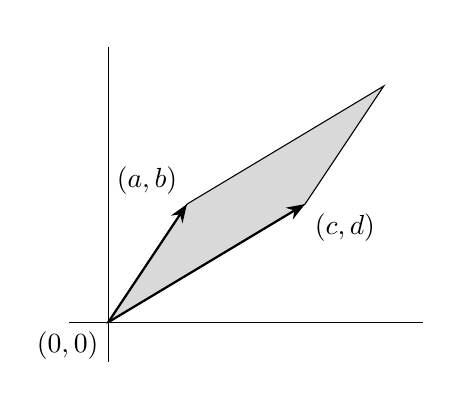
\begin{tikzpicture}
    % Define the scaled coordinates
    \coordinate (O) at (0,0);
    \coordinate (A) at (1, 1.5);   % (a,b)
    \coordinate (D) at (2.5, 1.5); % Changed from (2.5, 0.5) to make angle smaller
    \coordinate (B) at ($ (A) + (D) $); % This will now be (3.5, 3.0)

    % Draw the axes (no arrows), adjusted for the new coordinates
    \draw (-0.5,0) -- (4,0) node[right] {};
    \draw (0,-0.5) -- (0,3.5) node[above] {}; % Adjusted y-axis limit

    % Draw the parallelogram and fill it with gray
    \fill[gray!30] (O) -- (A) -- (B) -- (D) -- cycle;
    \draw (O) -- (A) -- (B) -- (D) -- cycle;

    % Add labels for the coordinates in math mode
    \node[below left] at (O) {$(0,0)$};
    \node[above left] at (A) {$(a,b)$};
    \node[below right] at (D) {$(c,d)$};

    % Add arrows for the vectors with -Stealth style
    \draw[-Stealth, thick] (O) -- (A);
    \draw[-Stealth, thick] (O) -- (D);
\end{tikzpicture}

\end{document}
